\documentclass{article}

\usepackage{amsmath}
\usepackage{amssymb}
\usepackage{tikz}
\usetikzlibrary{automata,positioning,arrows}
\tikzset{
	>=stealth',
	initial text=$ $
	}

\title{Assignment 5}
\date{2019-02-28}
\author{MONTGOMERY, BENNET 20074049 CISC223\\
		\and GOEL, CHRISTOPHER 20053408 CISC223\\
		\and VIOLO, JARED 20051382 CISC223\\
		\and DALLAS, SPENCER 20048480 CISC223}
		
\begin{document}
	\maketitle
	
	\section*{Q1.}
	This context free grammar is represented by a pushdown automata with the stack alphabet $\Gamma = \{A,C\}$ where two $A$ symbols are pushed for every $a$ in the input string, one $A$ symbol is popped for every $b$ in the input string, one $C$ symbol is pushed for every $c$ in the input string, and two $C$ symbols are popped for every $d$ in the input string. The precise pushdown automata diagram is:
		\begin{figure}[!h]
			\centering
			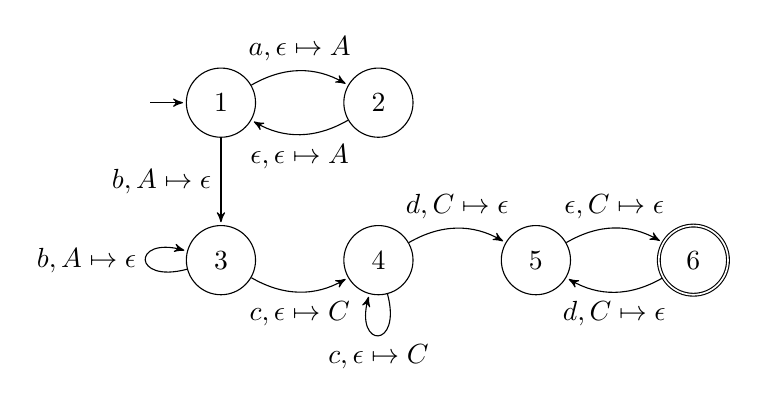
\begin{tikzpicture}[shorten >=1pt,node distance=2cm,on grid,auto]
				\node[state,initial] (1) {$1$};
				\node[state] (2) [right=of 1] {$2$};
				\node[state] (3) [below=of 1] {$3$};
				\node[state] (4) [right=of 3] {$4$};
				\node[state] (5) [right=of 4] {$5$};
				\node[state,accepting] (6) [right=of 5] {$6$};
				\path[->]
				(1) edge [bend left] node {$a, \epsilon \mapsto A$} (2)
					edge node [swap] {$b, A \mapsto \epsilon$} (3)
				(2) edge [bend left] node {$\epsilon, \epsilon \mapsto A$} (1)
				(3) edge [loop left] node {$b, A \mapsto \epsilon$} ()
					edge [bend right] node [swap] {$c, \epsilon \mapsto C$} (4)
				(4) edge [loop below] node {$c, \epsilon \mapsto C$} ()
					edge [bend left] node {$d, C \mapsto \epsilon$} (5)
				(5) edge [bend left] node {$\epsilon, C \mapsto \epsilon$} (6)
				(6) edge [bend left] node {$d, C \mapsto \epsilon$} (5);
 			\end{tikzpicture}
		\end{figure}
	\\The trace for processing $abbccccdd$ with the above pushdown automata is given in Table 1 on the following page.
	\newpage
		\begin{table}
			\caption{Trace Table}
			\centering
			\begin{tabular}{ c | c | c }
				\hline
				\hline	
				Current State & Current Input Remaining & Current Stack \\
				\hline
				1 & $abbccccdd$ & $\epsilon$ \\
				2 & $bbccccdd$ & $A$ \\
				1 & $bbccccdd$ & $AA$ \\
				3 & $bccccdd$ & $A$ \\
				3 & $ccccdd$ & $\epsilon$ \\
				4 & $cccdd$ & $C$ \\
				4 & $ccdd$ & $CC$ \\
				4 & $cdd$ & $CCC$ \\
				4 & $dd$ & $CCCC$ \\
				5 & $d$ & $CCC$ \\
				6 & $d$ & $CC$ \\
				5 & $\epsilon$ & $C$ \\
				6 & $\epsilon$ & $\epsilon$ \\
				\hline
			\end{tabular}
		\end{table}
	\section*{Q2}
	\subsection*{(a)}
	Assuming the language is context free, we let $l = m^{n+1}$ where $m$ is the max production length and $n$ is the number of non-terminal symbols, and we let $i = k = l$. This makes the string $a^lb^lc^l$. Since this string has a length greater than $m^{n+1}$, there must exist strings $u, v, w, x, y$ such that $uvwxy$ is $a^lb^lc^l$, $v \neq \epsilon$, $x \neq \epsilon$, and length($vwx$) $\leq l$. If this grammar is indeed context free, then the string $uv^kwx^ky$ must also be generated by the grammar for all $k, k \geq 0$. There are 3 possible cases for values of $v$ and $x$. If $v$ or $x$ consist of a string of only $b$ or $c$ characters (i.e. $b...b$, $c...c$), pumping $v$ and $x$ up will lead to either an inequality in the number of $b$ and $c$ characters or the number of $b$ or $c$ characters will exceed the number of $a$ characters in a string defined by the grammar, neither of which are allowed by the language. If either $v$ or $x$ consist of a string of only $a$ characters (i.e. $a...a$), pumping $k$ down to 0 will reduce the number of $a$ characters below the number of $b$ or $c$ characters, which is not allowed by the language. Finally, if $v$ or $x$ consist of a string of two unique characters (i.e. $a...ab...b$ or $b...bc...c$), pumping $k$ up will lead to a pattern of alternating $a$ and $b$ strings or alternating $b$ and $c$ strings, which is not allowed by the language. Since all possible values of $v$ and $x$ lead to a contradiction, the grammar is not context free.
	\subsection*{(b)}
	This language is described by the following context free grammar:
		\begin{align*}
			S &\rightarrow XY\\
			X &\rightarrow aaZbbccc \hphantom{a} | \hphantom{a} aaXccc\\
			Z &\rightarrow bbZ \hphantom{a} | \hphantom{a} \epsilon\\
			Y &\rightarrow ddY \hphantom{a} | \hphantom{a} dd
		\end{align*}
\end{document}